\documentclass[a4paper,12pt]{article}
\usepackage{a4wide}
\usepackage[pdftex]{hyperref}
\usepackage[german]{babel}
\usepackage[utf8]{inputenc}
\usepackage{amssymb}
\usepackage{csquotes}
\usepackage{wrapfig}
\usepackage{graphicx}
\usepackage{multicol}
\usepackage{amsmath}
\usepackage{enumitem}
\usepackage{polynom}
\usepackage{siunitx}

\setlength{\marginparsep}{1 cm}
\setlength{\topmargin}{-0.6in}
\setlength{\textheight}{9.5in}
\pagestyle{plain}

\polyset{%
   style=C,
   delims={\big(}{\big)},
   div=:
}

% Polynomial long division
\polyset{%
	style=C,
	delims={\big(}{\big)},
	div=:
}

% Differential operator
\newcommand{\diff}[1]{\:\mathrm{d}{#1}}
\newcommand{\pdd}[2]{\frac{\partial #1}{\partial #2}}
\newcommand{\pddn}[3]{\frac{\partial^{#1} #2}{\partial #3^{#1}}}
\newcommand{\dd}[2]{\frac{\mathrm{d}{#1}}{\mathrm{d}{#2}}}
\newcommand{\ddn}[3]{\frac{\mathrm{d}^{#1}{#2}}{\mathrm{d}{#3^{#1}}}}

% N-th root
% \nroot{3}{27}
\newcommand*{\nroot}[2]{\sqrt[\leftroot{-1}\uproot{2}#1]{#2}}
\newcommand*{\ncroot}[4]{\sqrt[\leftroot{#1}\uproot{#2}#3]{#4}}

% 2 component vector
% \tvect{1}{-1}
% \tvec{1}{-1}
\newcommand{\tvect}[2]{%
   \ensuremath{\Bigl(\negthinspace\begin{smallmatrix}#1\\#2\end{smallmatrix}\Bigr)}}
\newcommand{\tvec}[2]{%
    \ensuremath{\left(\negthinspace\begin{matrix}#1\\#2\end{matrix}\right)}}

% 3 component vector
% \rvect{1}{-1}{0}
% \rvec{1}{-1}{0}
\newcommand{\rvect}[3]{%
   \ensuremath{\Bigl(\negthinspace\begin{smallmatrix}#1\\#2\\#3\end{smallmatrix}\Bigr)}}
\newcommand{\rvec}[3]{%
    \ensuremath{\left(\negthinspace\begin{matrix}#1\\#2\\#3\end{matrix}\right)}}

% Long vector arrow
% \xshlongvec{ABC}

% German-style quotation marks %
\MakeOuterQuote{"}

% Number sets
\newcommand{\N}{\mathbb{N}}
\newcommand{\Z}{\mathbb{Z}}
\newcommand{\Q}{\mathbb{Q}}
\newcommand{\R}{\mathbb{R}}
\newcommand{\C}{\mathbb{C}}

\newcommand{\setzero}{\varnothing}

% Mention (small caps)
\newcommand{\mention}[1]{\textsc{#1}}

% Functions
\newcommand{\asin}[0]{\text{asin}}
\newcommand{\acos}[0]{\text{acos}}
\newcommand{\atan}[0]{\text{atan}}
\newcommand{\sgn}[0]{\text{sgn}}
\newcommand{\grad}[0]{\text{grad}}

% Scale
% Usage in math mode: \Scale[1.5]{...equation...} %
\newcommand*{\Scale}[2][4]{\scalebox{#1}{$#2$}}%

% Units
\newcommand{\um}{\text{m}}
\newcommand{\us}{\text{s}}
\newcommand{\ukm}{\text{km}}
\newcommand{\ukg}{\text{kg}}
\newcommand{\uh}{\text{h}}
\newcommand{\ukmh}{\frac{\ukm}{\uh}}
\newcommand{\umpers}{\frac{\um}{\us}}
\newcommand{\umss}{\frac{\ukm}{\us^2}}
\newcommand{\ukgss}{\frac{\ukg}{\us^2}}
\newcommand{\degrees}[1]{\SI{#1}{\degree}}

% Floor / ceil
\newcommand{\floor}[1]{\left\lfloor #1 \right\rfloor}
\newcommand{\ceil}[1]{\left\lceil #1 \right\rceil}

% Circle characters
\newcommand*\circled[1]{
    \tikz[baseline=(char.base)]{
        \node[shape=circle,draw,inner sep=2pt] (char) {#1};
    }
}



\begin{document}

\begin{center}
{\bf {\large Aufgabenblatt 6 (MI/IT)}}
\end{center}

\begin{enumerate}

\item
Nähern Sie die Funktion $\ln(x)$ durch ein Taylor-Polynom 3. Grades für die Entwicklungsstelle $x_0=3$ !


\item
Schätzen Sie den Wert von $\cos(89^{\circ})$ ! Ermitteln Sie hierzu die Taylorentwicklung 2. Ordnung von $\cos(x)$ an der Stelle $x_0=90^{\circ}$ und setzen Sie dann $x = 89^{\circ}$ in diese Taylorentwicklung ein! Nutzen Sie die Restgliedabschätzung für $R_3(x)$, um den Fehler des ermittelten Wertes abzuschätzen!



\item (*) Skizzieren Sie die zugehörigen Funktionsgraphen! Die Skizze soll qualitativ erfolgen, Maßstäblichkeit und eine Achsenbeschriftung ist (bis auf markante Punkte) nicht notwendig. Denken Sie dazu auch über die in Klammern stehenden Eigenschaften nach.
\begin{enumerate}
\item $\frac{1}{3}\sin(2x-\frac{3}{4}\pi)$ {\footnotesize[Skalierung, Verschiebung]}
\item $\sin(x^2)$ {\footnotesize[Symmetrie, Nullstellen]}
\item $e^\frac{1}{x}$ {\footnotesize[Verhalten für $x\to\pm\infty$, Funktionswerte in der linken und rechten Halbebene, Null/Extremstellen]}
\item $\sin^2(x)$ {\footnotesize[Wertebereich, Nullstellen, Periode]}
\item $\frac{1}{\sin(x)}$ {\footnotesize[Periode, Wertebereich]}
\end{enumerate}



\item Ermitteln Sie eine Stammfunktion durch Lösen folgender unbestimmter Integrale:
\begin{enumerate}
\begin{multicols}{2}
\item $\int \frac{1}{x} + \frac{1}{x^2} \d x$
\item $\int \cos(10x)\d x$
\item $\int x\cdot \sin(x^2) \d x$
\item $\int \frac{x}{\sqrt{2+x^2}} \d x$ ($u=x^2$)
\item $\int x \cdot e^x \d x$
\item $\int x^2 \cdot \ln(x) \d x$
\end{multicols}
\end{enumerate}



\item Flächenberechnung: Lösen Sie die folgenden bestimmten Integrale:
\begin{enumerate}
\begin{multicols}{2}
\item $\int\limits_1^3 x^2+ 4 $d$x$
\item $\int\limits_0^1 |2x-1|$d$x$
\end{multicols}
\end{enumerate}



\item
Bestimmen Sie den Wert dieser uneigentlichen Integrale, falls sinnvoll und möglich:
\begin{enumerate}
\begin{multicols}{2}
\item $\int\limits_2^5 \frac{1}{(x-3)^2}$d$x$
\item $\int\limits_2^3 \frac{1}{\sqrt{x-2}}$d$x$
\end{multicols}
\end{enumerate}



\item Ermitteln Sie den Flächeninhalt, welcher durch die Normalparabel $y=x^2$ und die Gerade $y=3$ begrenzt wird. Fertigen Sie hierzu zuerst eine Skizze an und ermitteln Sie dann die Fläche durch Integration!


\end{enumerate}

\newpage

Zusatzaufgabe:

Im Jahr 2002 hat es in Dresden extremes Hochwasser gegeben (siehe Abb. \ref{fig1}). Eine Maßnahme für den Hochwasserschutz besteht im Anlegen von Rückhaltebecken. 

Berechnen Sie für zwei nachfolgend beschriebene Szenarien näherungsweise das jeweils erforderliche Volumen. Verwenden Sie dafür das folgende mathematische Modell für die Durchflussgeschwindigkeit an der Messstelle Dresden:

$$v(t)=\frac{4500}{1+0,16t^2}+100$$

Dabei steht $t$ für die Zeit in Tagen und $v(t)$ für die Durchflussmenge in $\text{m}^3/\text{s}$ steht. An der Stelle $t=0$ befindet sich das Maximum  der Kurve. Finden Sie auch eine Veranschaulichung der berechneten Volumina.

\begin{enumerate}[label=(\roman*)]

\item Szenario 1: Begrenzung der Durchflussgeschwindigkeit auf $1710\, \text{m}^3/\text{s}$ (die im Zeitraum $t=-3,3..3,3\,\text{d}$
überschritten wurde).

\item Szenario 2: Begrenzung der Durchflussgeschwindigkeit auf $333\, \text{m}^3/\text{s}$ (die im Zeitraum $t=-10,7..10,7\,\text{d}$
überschritten wurde).

\end{enumerate}

Hinweis: Bei der Integration ist auf die Einheiten zu achten. $\int \frac{1}{x^2+1}$d$x=$atan$(x)+C$

\begin{figure}[ht]
	\centering
  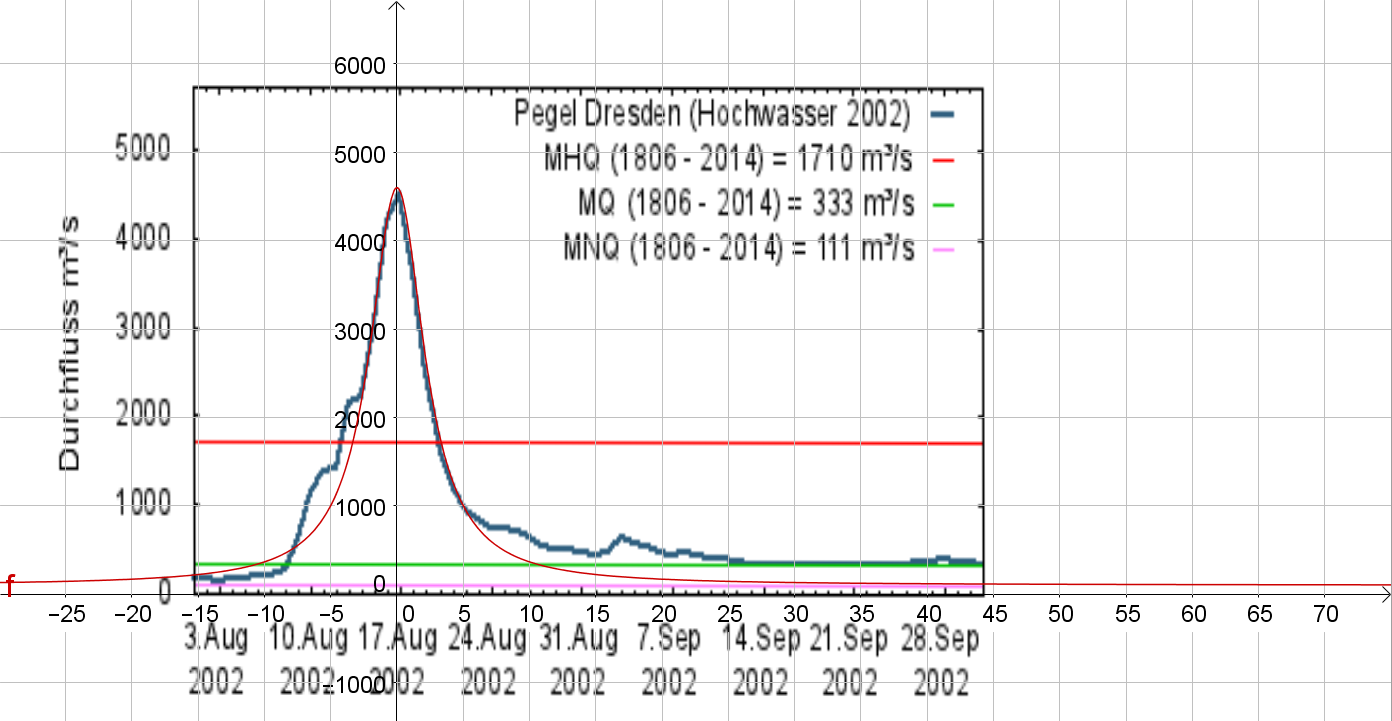
\includegraphics[width=0.65\textwidth]{../pool/ex-fn-model-1-img-a.png}
	\caption{Durchflussdaten zum Hochwasser des Jahres 2002 in Dresden mit Modellkurve; MHQ: Mittlerer Hochwasserabfluss, MQ: Mittlerer Abfluss, MNQ: Mittlerer Niedrigwasserabfluss in betrachteter Zeitspanne }
	\label{fig1}
\end{figure}



\newpage

\begin{center}
{\bf {\large Lösungen}}
\end{center}

\begin{enumerate}

\item $f(x) = \ln(x)$. Ableiten

$$f'(x) = \frac{1}{x}$$
$$f''(x) = -\frac{1}{x^2}$$
$$f'''(x) = \frac{2}{x^3}$$

Für die Entwicklungsstelle $x_0 = 3$:

$$f(3) = \ln(3)$$
$$f'(3) = \frac{1}{3}$$
$$f''(3) = -\frac{1}{9}$$
$$f'''(3) = \frac{2}{27}$$

Damit folgt für die Taylorentwicklung 3. Grades:

$$\ln(x) \approx \ln(3) + \frac{1}{3} (x-3) - \frac{1}{18} (x-3)^2 + \frac{1}{81} (x-3)^3$$

Anmerkung: $f''''(x)=\frac{6}{x^4}$. Für $\Delta x \in [0,3)$ ist $\max\limits_{\vartheta\in[3-\Delta x,3+\Delta x]}|f''''(\vartheta)| = \frac{6}{(3-\Delta x)^4}$. Das Restglied kann dann abgeschätzt werden mit $|R_3(x)| \leq \frac{|x-3|^4}{4!} \frac{6}{(3-|x-3|)^4}$.



\item Als Funktion betrachten wir $f(x) = \cos(x)$ und entwickeln um $x_0=90^\circ = \frac{\pi}{2}$:

$$f'(x) = -\sin(x)$$
$$f''(x) = -\cos(x)$$
$$f'''(x) = \sin(x)$$

Wir erhalten:

$\cos(x) \approx 0 + \frac{-1}{1!} (x-\frac{\pi}{2}) + \frac{0}{2!}(x-\frac{\pi}{2})^2 = -(x-\frac{\pi}{2})$

$\implies \cos(89^\circ) \approx \frac{\pi}{180} \approx 0,017453$

Da die zweite Ableitung $f''(\frac{\pi}{2})=0$ ist, stellt die Tangente gleichzeitig auch die Schmiegeparabel dar.

Anmerkung: Mit der Restgliedabschätzung folgt unter Verwendung von $\max\limits_{\vartheta \in [89^\circ,90^\circ]}|f^{(3)}(\vartheta)| = 1$ für den Höchstfehler $|R_3(x)| \leq \frac{(\frac{\pi}{180})^3}{3!}\cdot 1 \approx 0,000001$. Also $\cos(89^\circ) \in [0,017452;0,017454]$. Der tatsächliche Wert ist $\cos(89^\circ) = 0.01745240643...$



\item Im Folgenden kurz die Überlegungen, die man anstellen sollte, um den jeweiligen Graph skizzieren zu können. Eine Skizze der Graphen befindet sich am Ende.

\begin{enumerate}

\item Umschreiben als: $f(x) = \frac{1}{3}\sin(2(x-\frac{3}{8}\pi))$

Sinusfunktion, die (i) um $\frac{3}{8}{\pi}$ ($67,5^\circ$) nach rechts verschoben ist, (ii) entlang der x-Achse um den Faktor 2 gestaucht und (iii) entlang der y-Achse um den Faktor $3$ gestaucht ist.

\item $f(x) = \sin(x^2)$

Sinusfunktion, deren Argument immer stärker steigt, somit wird die Periode für betragsmäßig große Argument immer kleiner, die Sinusfunktion oszilliert also immer schneller. Wegen $f(x) = f(-x)$ ist die Funktion gerade, also symmetrisch bzgl. der y-Achse. Zudem $f(0) = 0$, der Graph beginnt im Ursprung.

\item $f(x) = e^\frac{1}{x}$

Wir überlegen uns einige wesentliche Eigenschaften der Funktion. Sie hat keine Nullstellen. $f'(x)=-\frac{1}{x^2}e^\frac{1}{x}$, also auch keine Extremstellen. Für $x=0$ ist die Funktion nicht definiert. Nahe dieser Stelle ist $\lim\limits_{x\to 0^{-}} e^\frac{1}{x} = 0$ und $\lim\limits_{x\to 0^{+}} e^\frac{1}{x} = \infty$. Das Verhalten im Unendlichen ist $\lim\limits_{x\to\pm\infty} e^\frac{1}{x} = e^0 = 1$.

Folglich geht der Graph für $x < 0$ im Ursprung los und nähert sich mit kleiner werdenden x-Werten der Gerade $y=1$ an. Für $x > 0$ kommt der Graph aus dem Positiv-Unendlichen und nähert sich $y=1$ an.

\item $f(x)=\sin^2(x)$

Da quadriert wird, werden alle negativen Werte ins Positive gebracht, damit ist die Periode halb so groß, also $\pi$. Alle Werte des Sinus sind betragsmäßig $\le 1$, werden durch das Quadrieren also kleiner, sodass der Graph zugespitzt wird.

\item $f(x)=\frac{1}{\sin(x)}$

Gleiche Periode wie Sinusfunktion, also $2\pi$. Die Nullstellen werden zu Polstellen. Bei der Nullstelle bei $0^\circ$ geht der Graph  links davon ins Negative-Unendliche und kommt rechts davon aus dem Positiv-Unendlichen. Bei der Nullstelle $180^\circ$  ist es umgekehrt: links davon geht der Graph ins Positiv-Unendliche, rechts davon kommt er aus dem Negativ-Unendlichen.

Bei $90^\circ$ gibt es ein lokales Minima mit $f(90^\circ) = \frac{1}{\sin(90^\circ)} = 1$ (da $\frac{1}{\sin(x)}$ am kleinsten wenn $\sin(x)$ am größten) und bei $270^\circ$ ein lokales Maxima mit $f(270^\circ) = -1$.

\end{enumerate}



\item

\begin{enumerate}

\item $\int \frac{1}{x} + \frac{1}{x^2}\d x = \ln(|x|)-\frac{1}{x}+C$

\item $\int \cos(10x)\d x = \frac{1}{10}\sin(10x) + C$

\item $\int x\cdot \sin(x^2)\d x \stackrel{\text{Substitution } z=x^2}{=} \frac{1}{2}\int \sin(z)\d z = -\frac{1}{2}\cos(x^2)+C$

\item Mit der Substitution $u=x^2$, $\d{x} = \frac{\d{u}}{2x}$ ergibt sich \\
$\int \frac{x}{\sqrt{2+x^2}} \d x = \int \frac{x/(2x)}{\sqrt{2+u}} \d u = \frac{1}{2} \int \frac{1}{\sqrt{2+u}} \d u = \frac{1}{2} \cdot 2 \cdot \sqrt{u+2} + C = \sqrt{x^2+2} + C$

\item $\int x \cdot e^x \d x = x e^x - \int e^x = x e^x - e^x = (x-1)\cdot e^x$

\item $\int x^2 \ln(x) \d x = \frac{x^3}{3}\ln(x) - \int \frac{x^3}{3}\cdot \frac{1}{x} \d x = \frac{x^3}{3}\ln(x) - \int \frac{x^2}{3} \d x$ \\
$ = \frac{x^3}{3}\ln(x) - \frac{x^3}{9} + C = \frac{1}{9}x^3 \cdot (3\ln(x)-1) + C$

\end{enumerate}



\item

\begin{enumerate}
\item $\int\limits_1^3 x^2+ 4 \d x = \lbrack \frac{x^3}{3}+4x\rbrack_1^3 = \frac{50}{3}$
\item Man fertigt eine Skizze an und erkennt, dass der zu berechnende Flächeninhalt durch 2 gleichgroße rechtwinklige Dreiecke begrenzt wird. Die Katheten haben die Längen $\frac{1}{2}$ und $1$. Somit $\int_0^1 |2x-1|\d x = \frac{1}{2}$.
\end{enumerate}



\item

\begin{enumerate}
\item $\int\limits_2^5 \frac{1}{(x-3)^2}\d x = \int\limits_{-1}^2 \frac{1}{x^2} \d x \stackrel{\text{def}}{=} \lim\limits_{\epsilon\to 0^{+}} (\int\limits_{-1}^{-\epsilon} \frac{1}{x^2} \d x + \int\limits_{\epsilon}^5 \frac{1}{x^2}\d x) = \lim\limits_{\epsilon\to 0^{+}} (\frac{2}{\epsilon} - \frac{3}{2})$

Dieser Grenzwert konvergiert nicht, daher hat das uneigentliche Integral keinen Hauptwert.

\item $\int\limits_2^3 \frac{1}{\sqrt{x-2}}\d x = \int\limits_0^1 \frac{1}{\sqrt{x}}\d x \stackrel{\text{def}}{=} \lim\limits_{\epsilon\to 0^{+}} \int\limits_\epsilon^1 \frac{1}{\sqrt{x}} = \lim\limits_{\epsilon\to 0^{+}}(2-2\sqrt{\epsilon}) = 2$
\end{enumerate}



\item Aus einer Skizze erkennt man, welche Berechnungen vorzunehmen sind. Die Integrationsgrenzen ergeben sich aus dem Schnittpunkt von $f(x)=x^2$ und $g(x)=3$:

$$x^2-3=0$$
$$\implies x_{1,2} = \pm \sqrt{3}$$

Aufgrund der Symmetrie reicht es aus, den positiven Teil $x \geq 0$ zu betrachten. Wir berechnen den Flächeninhalt zwischen x-Achse mit $f(x)$ und ziehen das Ergebnis anschließend vom Flächeninhalt des Rechtecks ab, welches durch den Ursprung und dem positiven Schnittpunkt von $f$ mit $g$ augespannt wird.

Das Rechteck hat den Flächeninhalt $A_\square = 3 \sqrt{3}$. Für den anderen Flächeninhalt ergibt sich:

$$\int_0^{\sqrt{3}} x^2 \diff{x}= \frac{1}{3} \lbrack x^3 \rbrack_0^{\sqrt{3}} = \frac{1}{3} (3\sqrt{3}-0) = \sqrt{3}$$

Somit ist der positive Anteil des Flächeninhalts innerhalb der Parabel $3\sqrt{3}-\sqrt{3}=2\sqrt{3}$ und der gesamte Flächeninhalt das Doppelte davon, also $4\sqrt{3}$.



\end{enumerate}

Zusatzaufgabe:

Sei $v(t)$ die Durchflussgeschwindigkeit in $\frac{m^3}{s}$, $t$ die Zeit in Tagen. Dann ist
$$V(t_0) = \int\limits_{-t_0}^{t_0}v(t)\d t$$

das Volumen an Wasser, welches in der Zeit zwischen $-t_0$ und $+t_0$ durchgeflossen ist. Für die Einheit ergibt sich

$$[V] = [v]\cdot[t] = \frac{m^3}{s}\cdot d = \frac{1000 dm^3}{s}\cdot 86400s = 86.400.000\cdot l$$

Zur Integration substituieren wir $z=0,4t$, um das Integral in Standardform zu bringen:

$$\int \frac{\d t}{1+0.16t^2} = \frac{1}{0,4}\int\frac{\d z}{1+z^2} = \frac{\text{atan}(0,4t)}{0,4} + C$$

Für das zu berechnende Volumen ziehen wir die Grenze der Durchflussgeschwindigkeit $\tau$ ab und erhalten für das komplette Integral:

$$\int\frac{4500}{1+0,16t^2}+ (100-\tau) \d t = \frac{4500}{0,4} \text{atan}(0,4t) + (100-\tau)t + C$$

Man beachte, dass $v(t)$ gerade ist und die Stammfunktion (für $C=0$) bei $t=0$ verschwindet; dies erleichtert die Rechnung.

\begin{enumerate}[label=(\roman*)]

\item Es ist $\tau=1710$. Gesucht ist $V(3,3) = \int_{-3,3}^{3,3} v(t) \d t$. Mit eingesetzten Werten ergibt sich für das Ergebnis der Zahlenwert  $\approx 21415$. In Einheiten entspricht dies $10129\cdot 86400000l \approx 8,8 \cdot 10^{11} \cdot l = 880 \text{ Millionen } m^3$ Dies entspricht etwa dem Volumen von $340$ Cheops-Pyramiden oder knapp dem Volumen des Bielersees ($1300 \text{ Millionen } m^3$).

\item $\tau=333$. Es ergibt sich $V(10,7) = \int_{-10,7}^{10,7} v(t) \d t = 25192$. In Einheiten also $2,2\cdot10^{12}\cdot l = 2,2 km^3$. Dies entspricht knapp dem Fassungsvermögen des Starnberger Sees ($3,0 km^3$).

\end{enumerate}



\end{document}

